% ==============================================================================
% Section 4b: Site-Level Dynamics and the Oasis Question
% ==============================================================================

\subsection{Site-Level Dynamics: Oasis Sites and the Geography of Persistence}
\label{sec:oasis}

The regional recovery percentages presented above conceal a fundamental question:
when a region ``recovers,'' does this reflect broad-based persistence across
many sites, or the survival of a few ``oasis'' sites that sustain most of the
regional population?  The answer, it turns out, depends dramatically on latitude
and has direct implications for conservation monitoring and reintroduction strategy.

\subsubsection{The Oasis Pattern in Oregon}

Oregon's apparent endpoint recovery (17.6\% snapshot in 2050, though 5-year 
average is only 5.4\% due to boom-bust cycles) masks an extreme concentration 
of survivors in oasis sites.  Across three
independent simulation seeds, Oregon's final population is overwhelmingly
concentrated in a handful of sites:

\begin{itemize}
  \item Only 17--21 of 59 Oregon sites retain any population at all by 2050
    (29--36\% of sites)
  \item The top 3 sites hold 39--79\% of the regional population (mean $\approx$ 54\%)
  \item The Gini coefficient for within-region population distribution reaches
    0.85--0.92 by 2050, compared to 0.00 at the start of the simulation

% --- Figure: Oasis Concentration ---
\begin{figure}[!htbp]
    \centering
    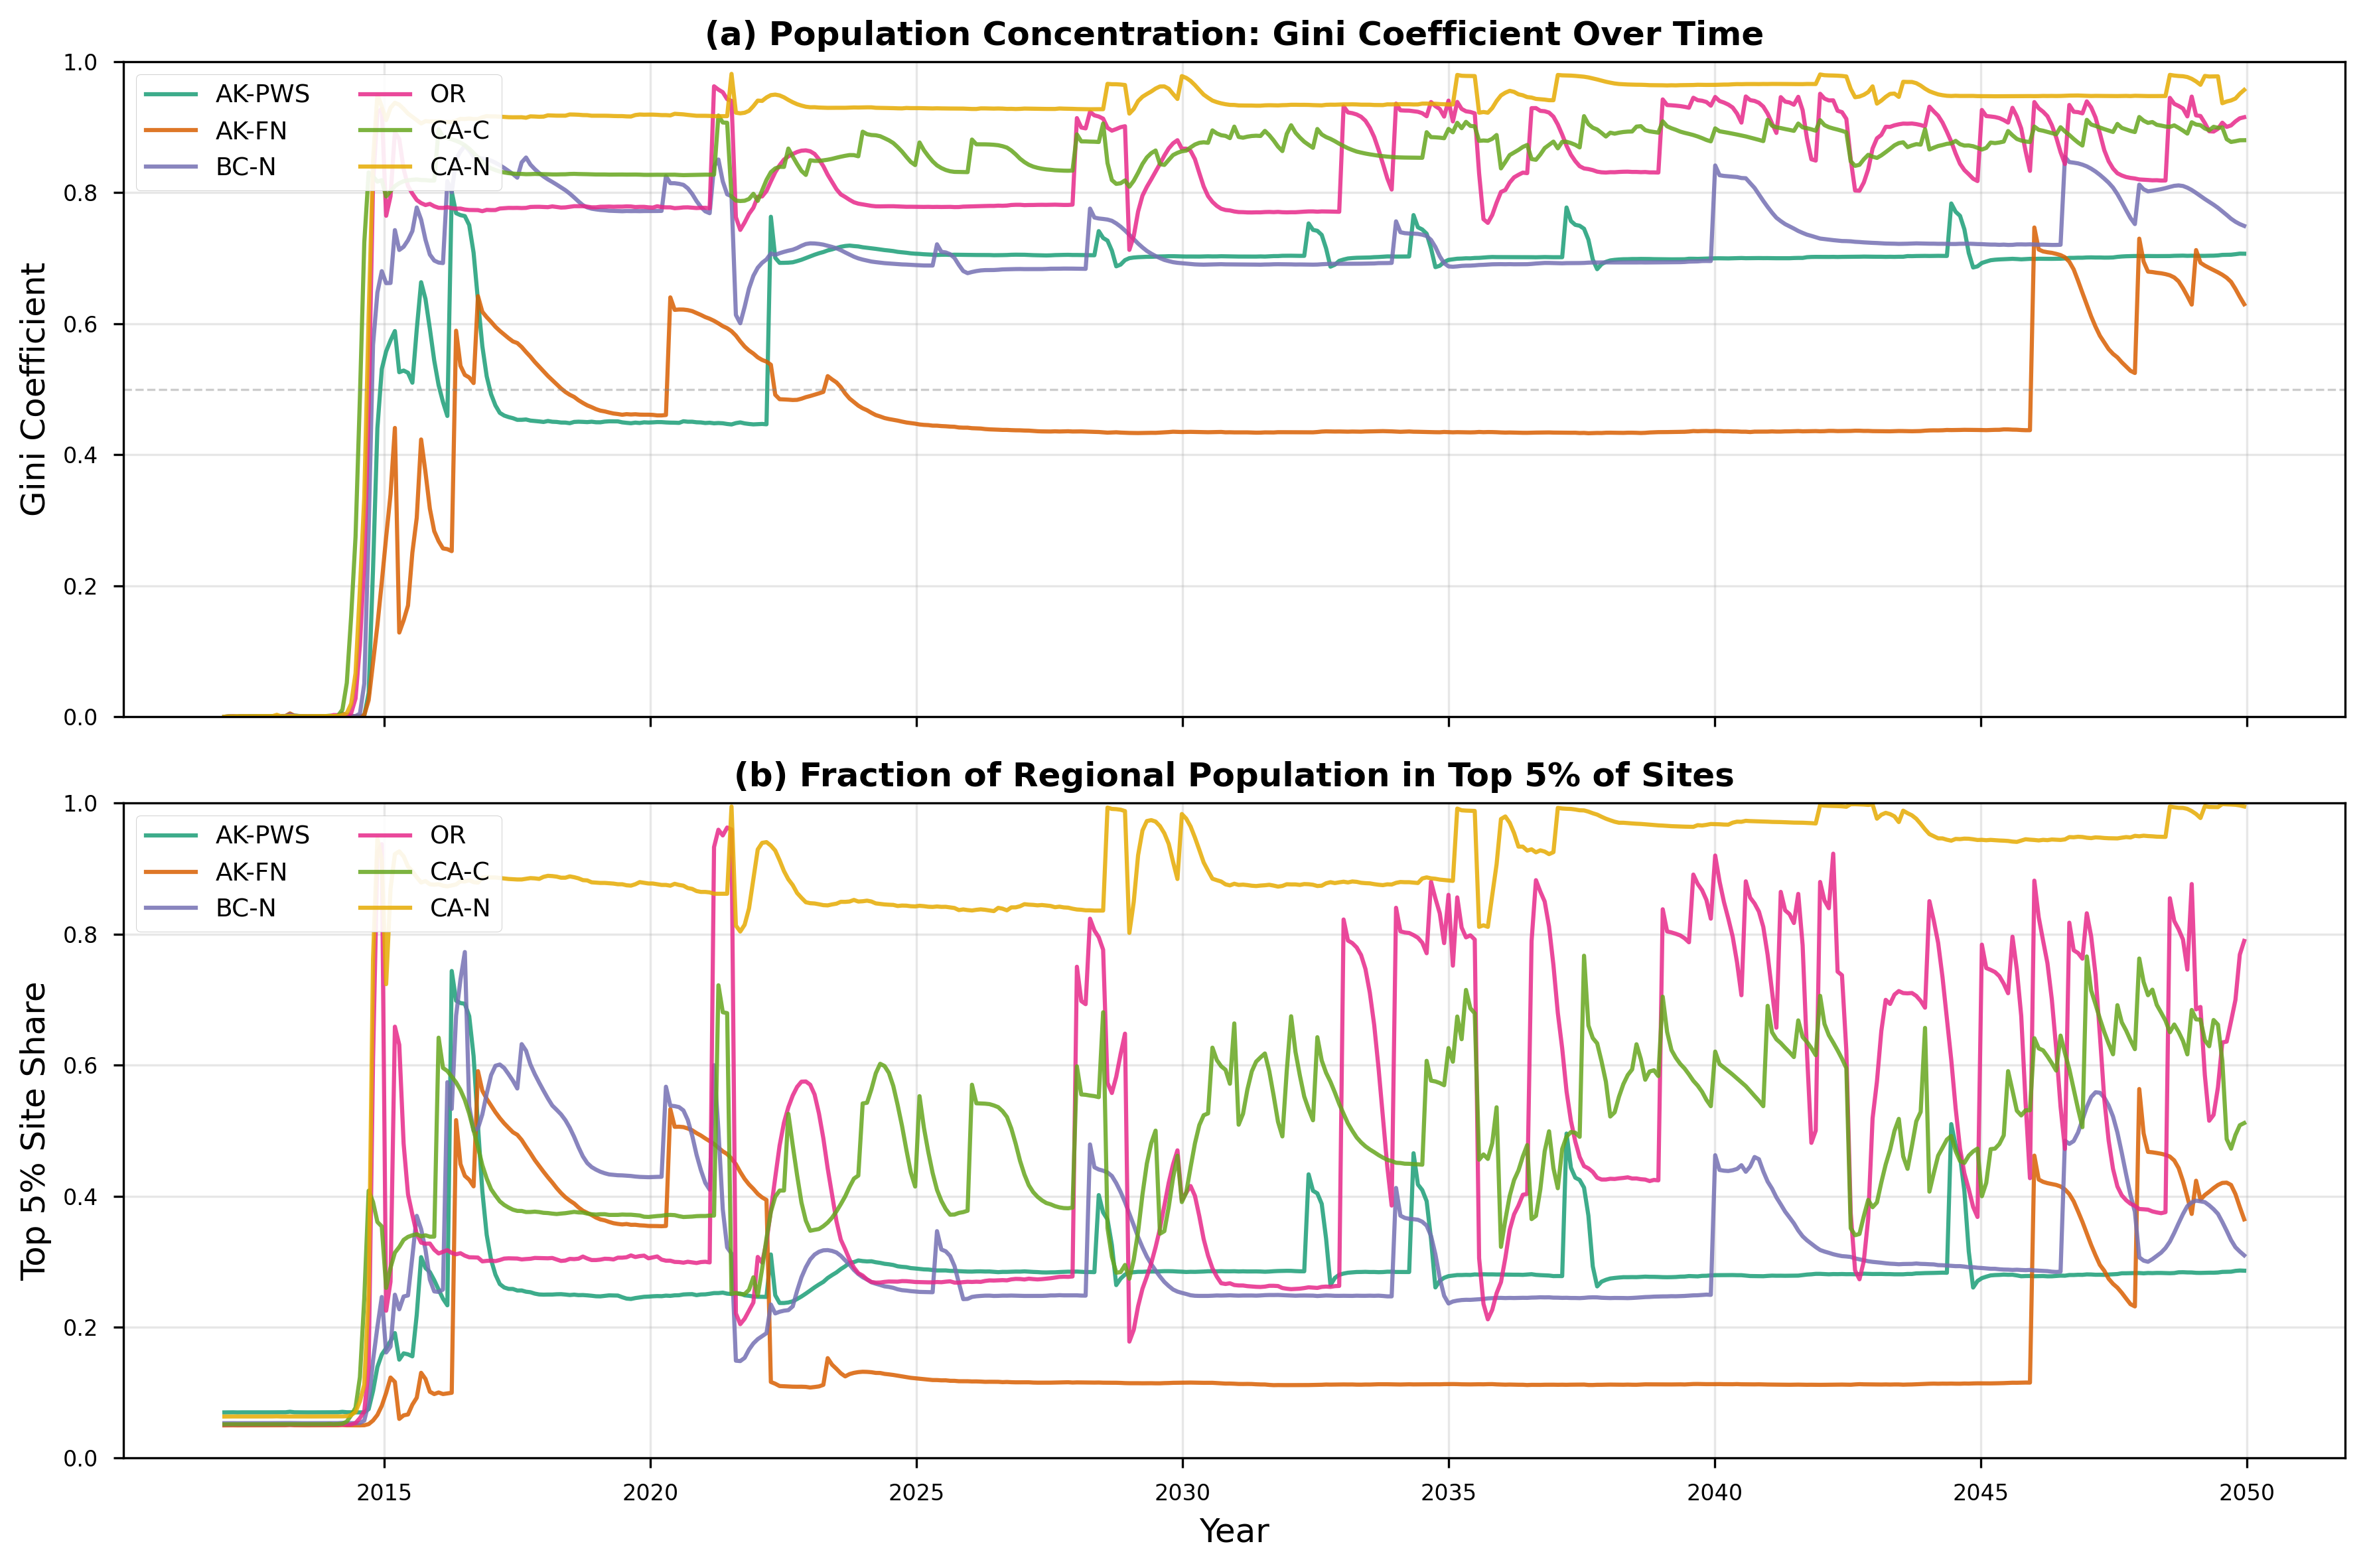
\includegraphics[width=0.80\textwidth]{figures/fig_oasis_concentration.png}
    \caption{Population concentration metrics over time for six key regions. \textbf{Left:} Gini coefficient of within-region site-level population distribution (0 = perfectly equal, 1 = all population in one site). Oregon (Gini $>$ 0.85 by 2050) shows extreme oasis concentration; AK-PWS and AK-FN (Gini $\approx$ 0.65) maintain distributed populations. \textbf{Right:} Fraction of regional population held by the top 3 sites over time. In Oregon, the top 3 sites hold 40--80\% of the population throughout the forecast period, while in Alaska they hold only 25--30\%.}
    \label{fig:oasis_concentration}
\end{figure}
    (Figure~\ref{fig:oasis_concentration})
\end{itemize}

\noindent
This concentration develops progressively over the simulation.  Pre-disease
(2012), population is uniformly distributed across all 59 sites at carrying
capacity ($K = 5{,}000$ each, Gini $= 0.00$).  By 2016, the post-crash population
is already uneven (Gini $\approx 0.78$), with only 38 sites retaining any
individuals.  By 2028, the oasis pattern is fully established: Gini exceeds
0.90, and the top 3 sites hold $\sim$80\% of the regional total
(Figure~\ref{fig:oasis_concentration}).

% --- Figure: Site Decomposition (oasis analysis) ---
\begin{figure}[!htbp]
    \centering
    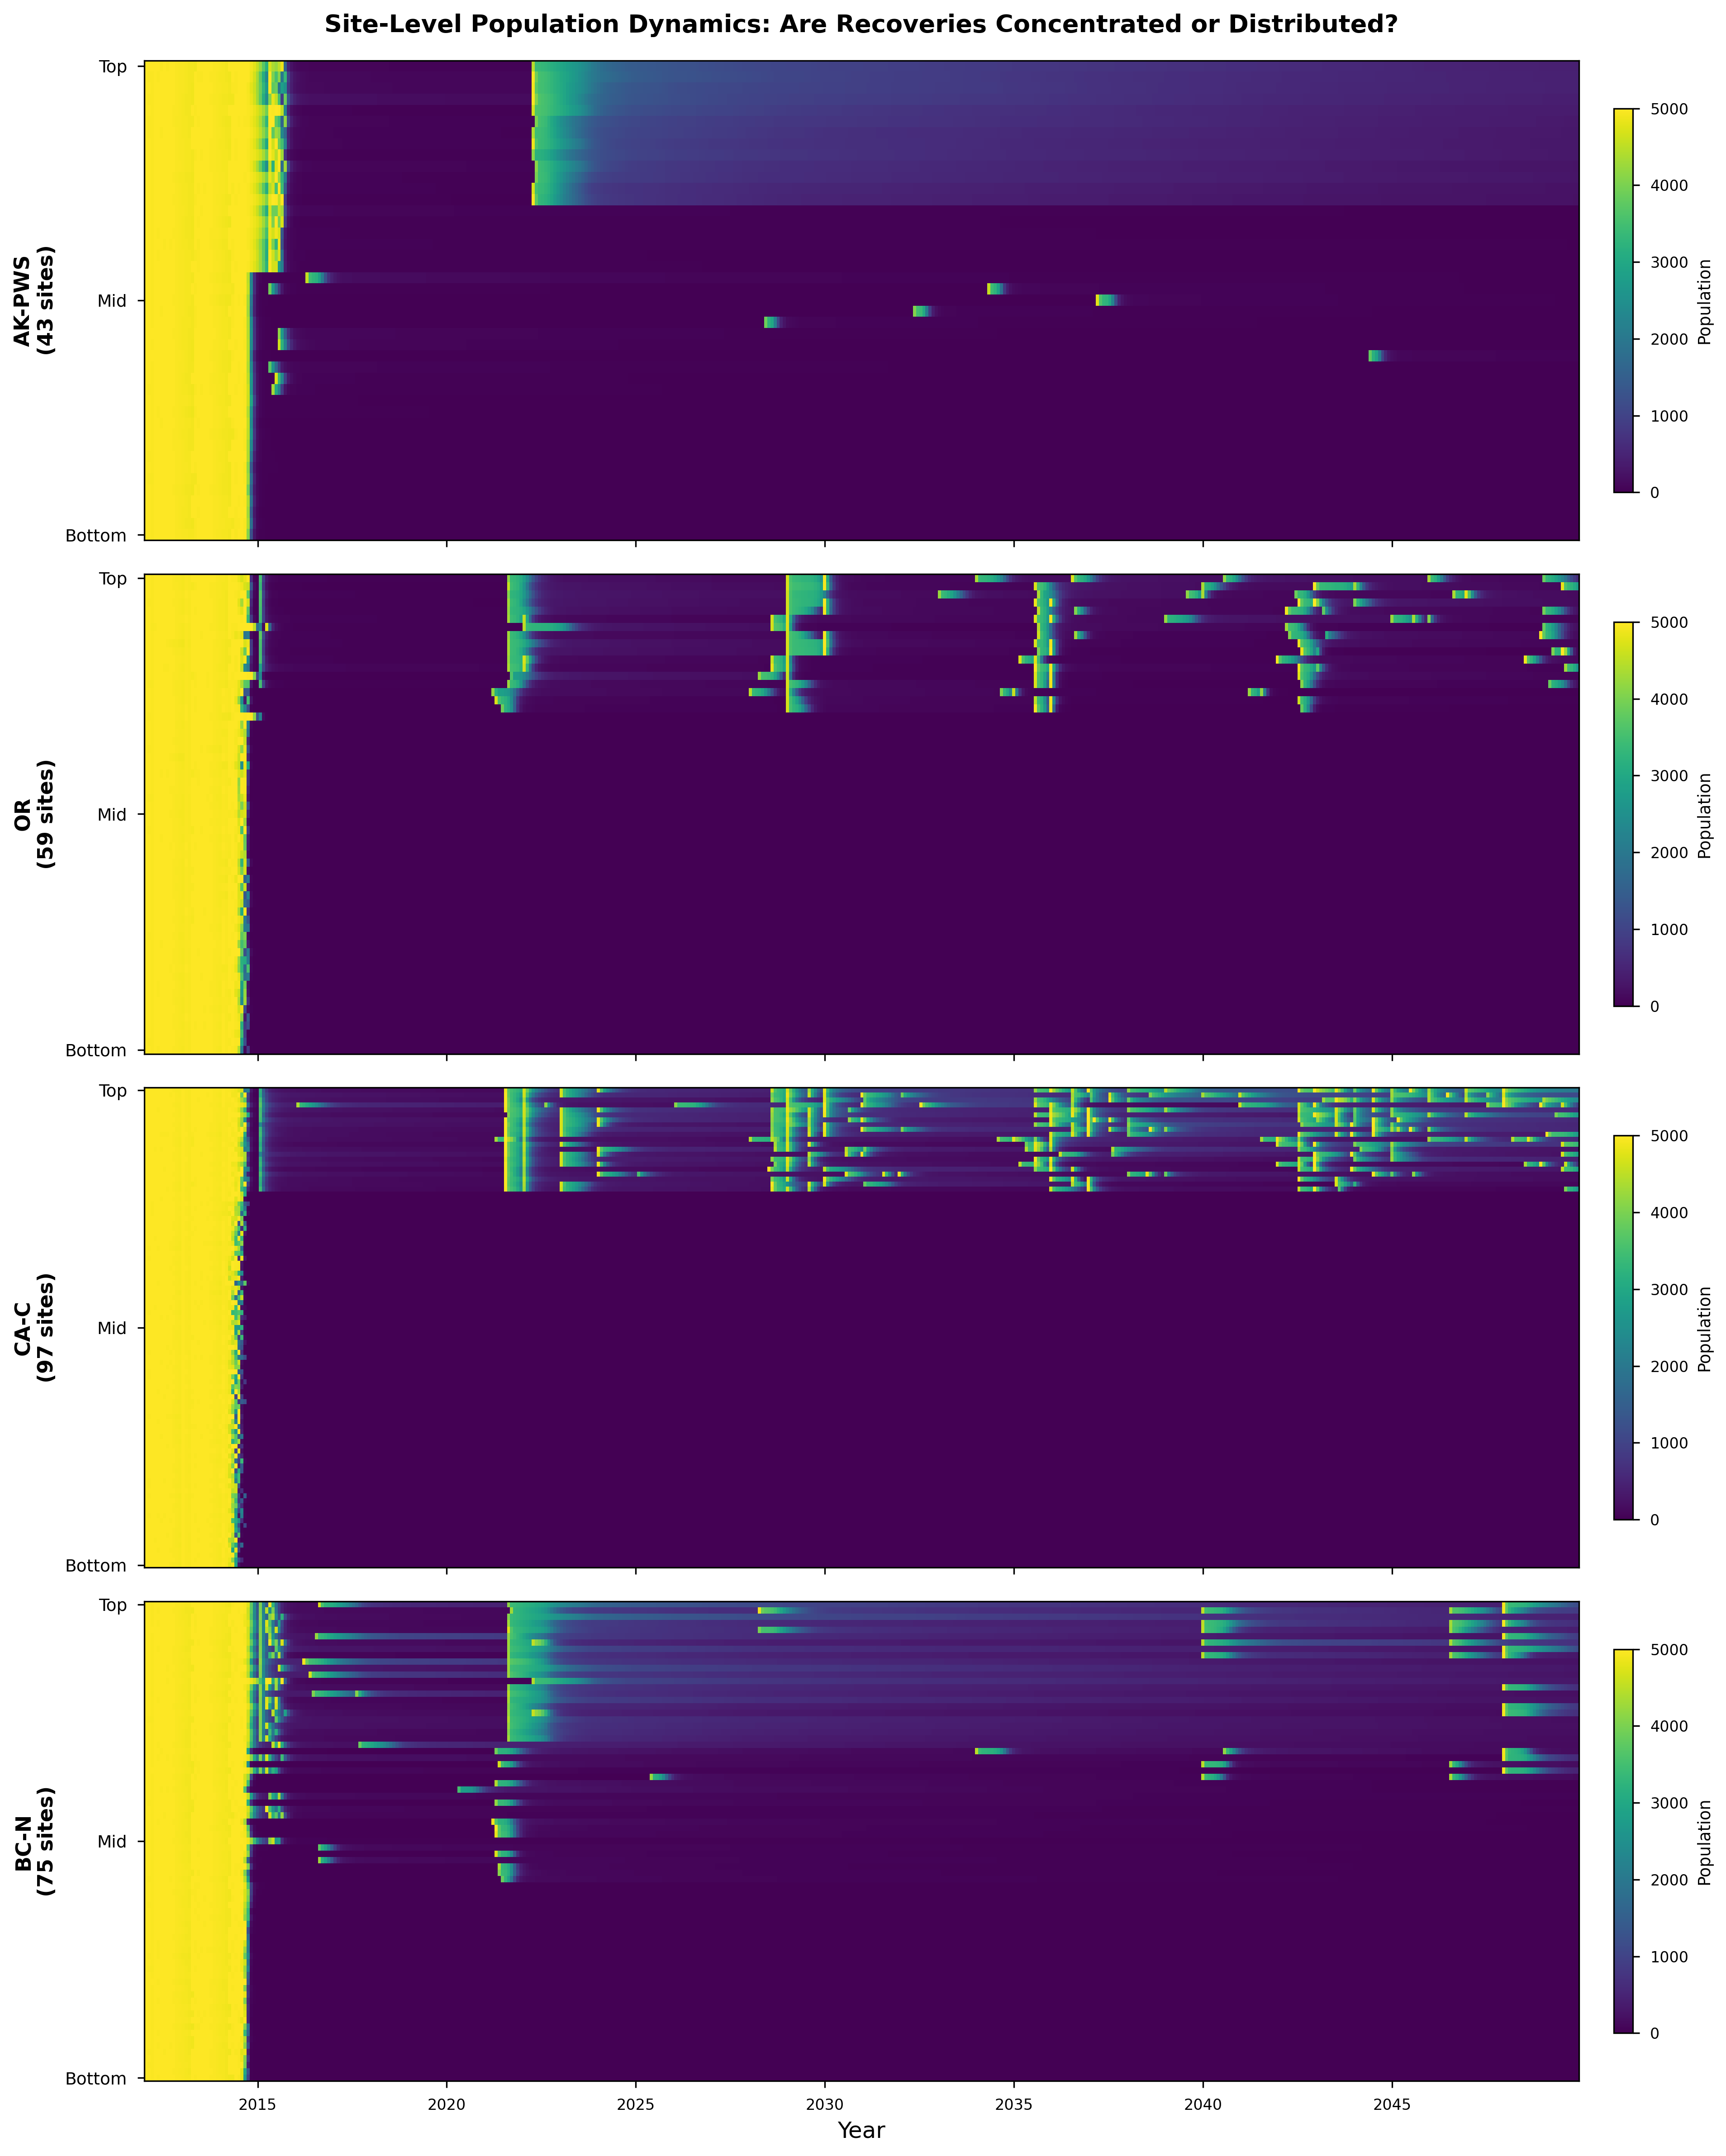
\includegraphics[width=0.85\textwidth]{figures/fig_site_decomposition.png}
    \caption{Site-level population dynamics within four key regions under the baseline scenario (F01, seed 42). Each panel shows the population trajectory of individual sites (thin lines) against the regional total (thick black line). In Oregon and CA-C, a handful of ``oasis'' sites hold the majority of the population, while in AK-PWS and AK-FN, population is broadly distributed across many sites. The boom-bust cycles visible at the regional level are driven by different subsets of sites in each cycle.}
    \label{fig:site_decomposition}
\end{figure>

% --- Figure: Oasis Concentration ---
\begin{figure}[!htbp]
    \centering
    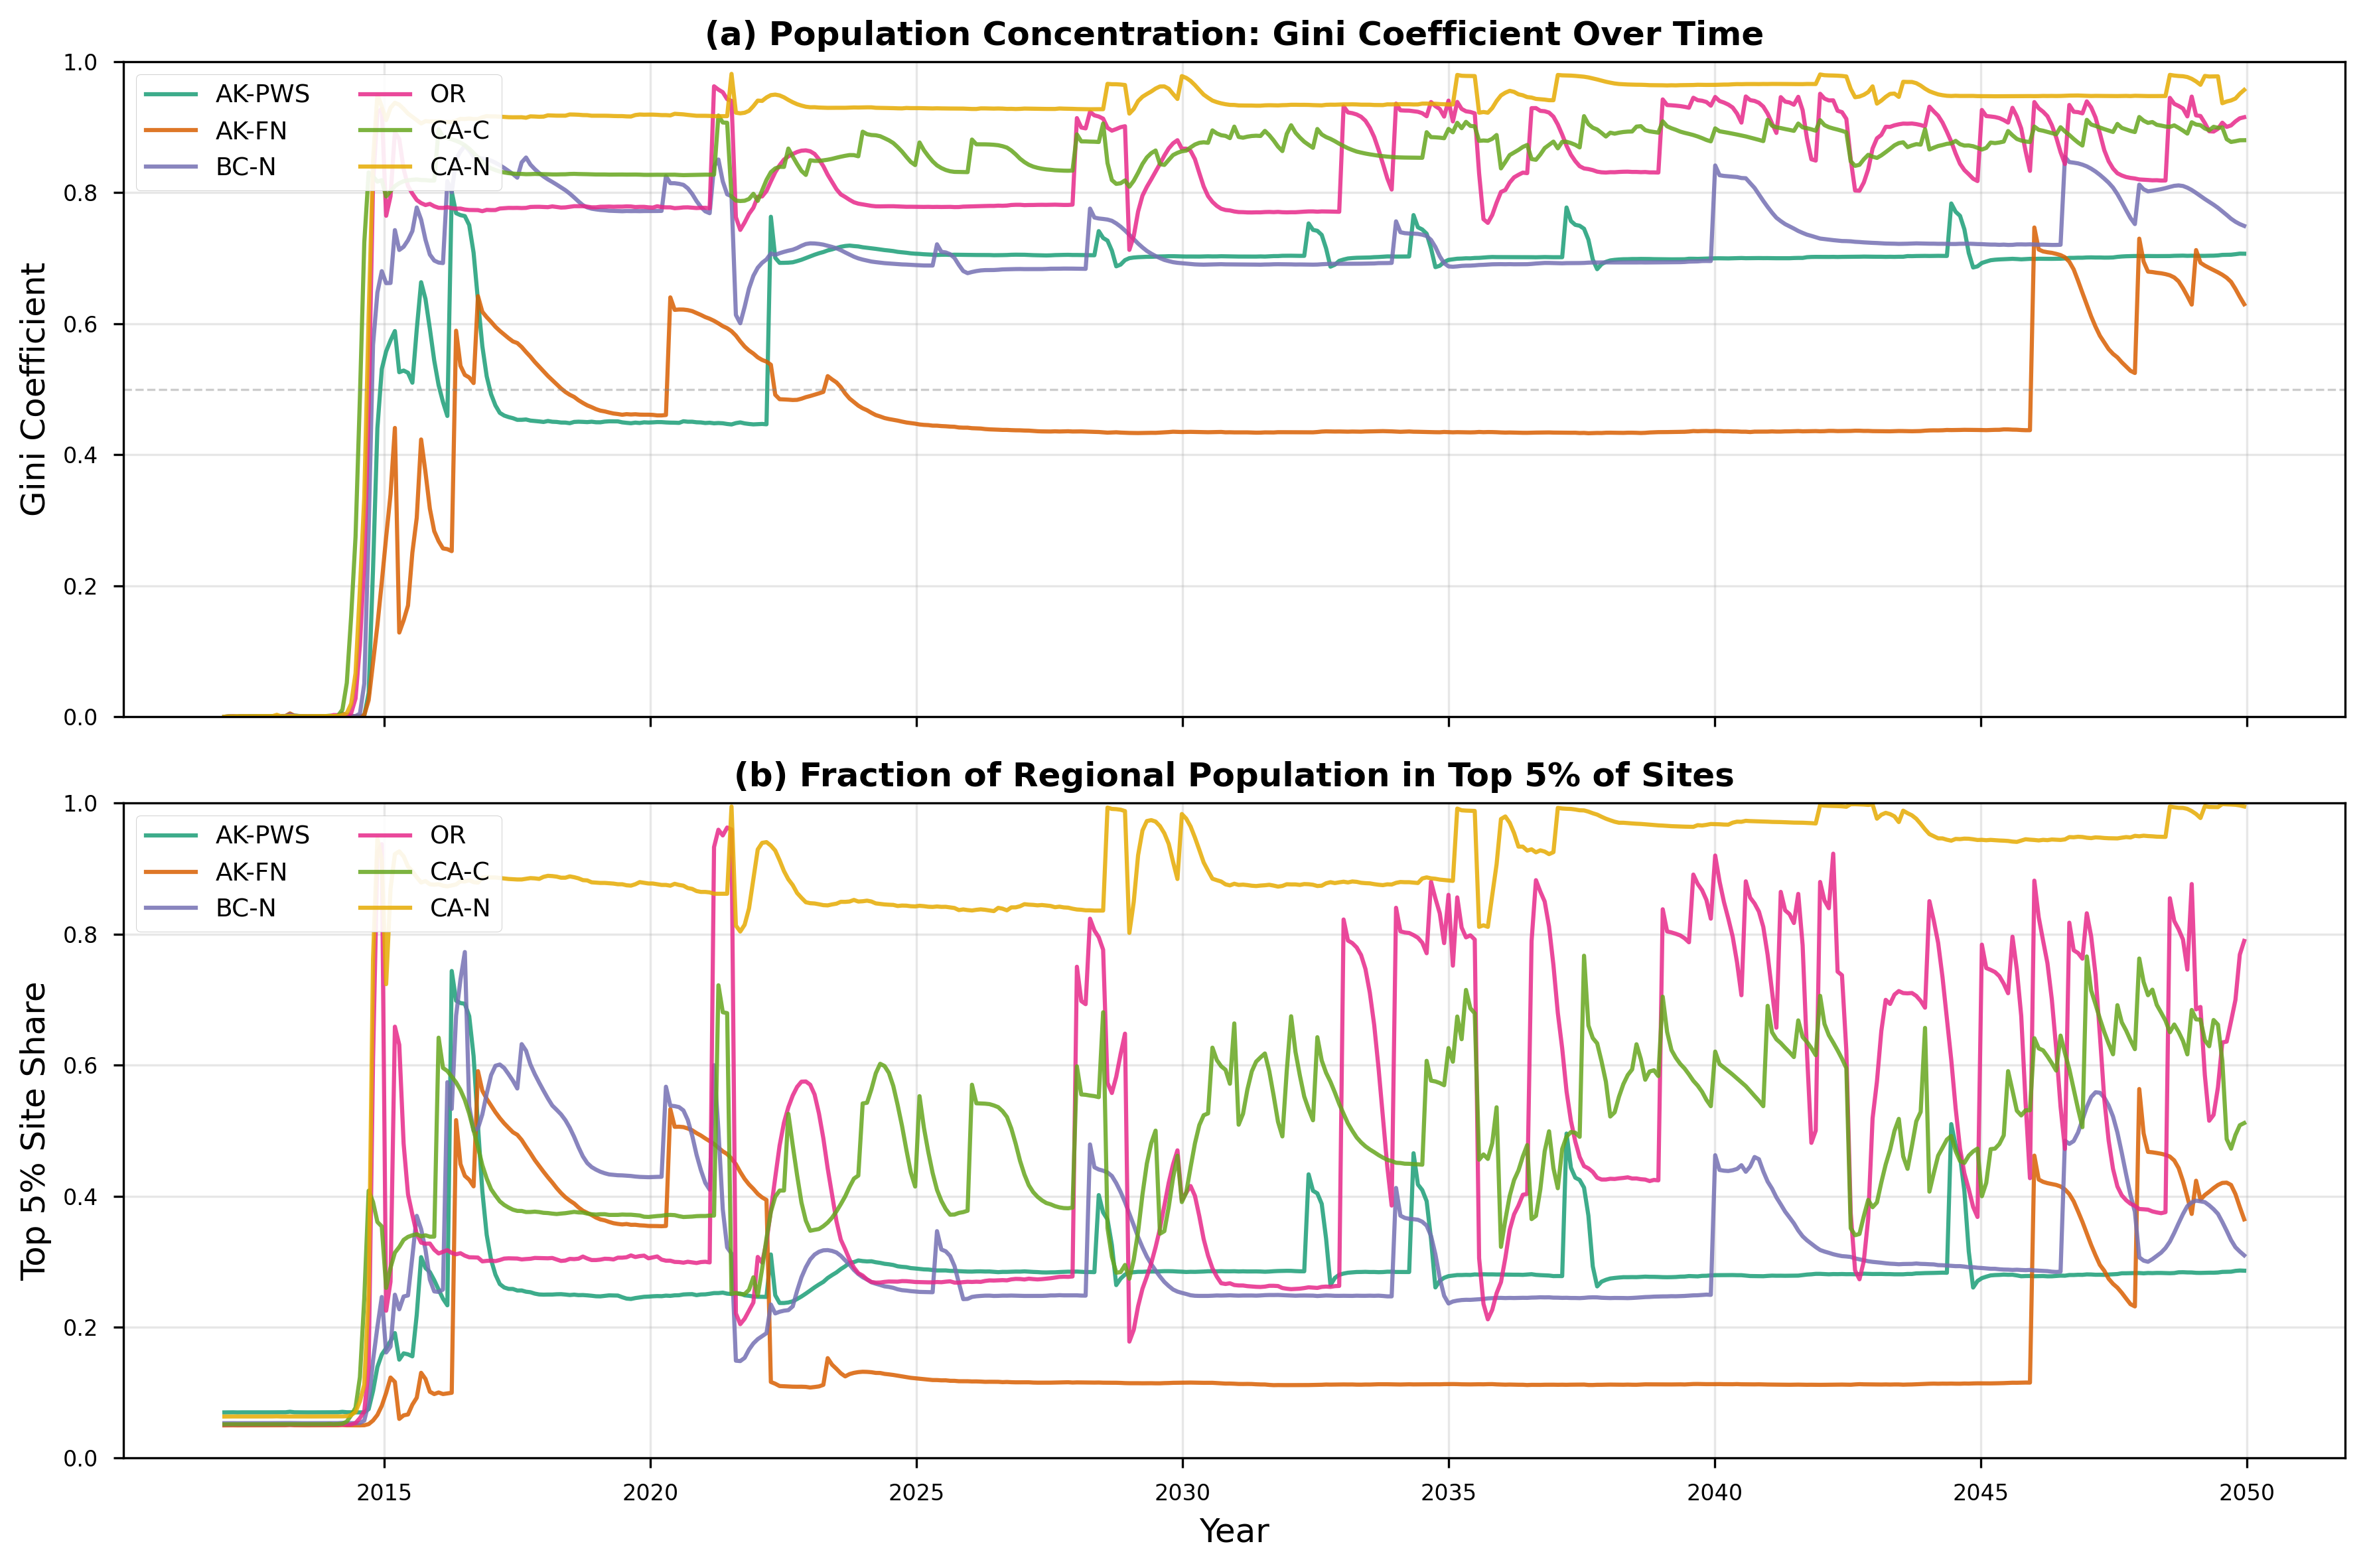
\includegraphics[width=0.80\textwidth]{figures/fig_oasis_concentration.png}
    \caption{Population concentration metrics over time for six key regions. \textbf{Left:} Gini coefficient of within-region site-level population distribution (0 = perfectly equal, 1 = all population in one site). Oregon (Gini $>$ 0.85 by 2050) shows extreme oasis concentration; AK-PWS and AK-FN (Gini $\approx$ 0.65) maintain distributed populations. \textbf{Right:} Fraction of regional population held by the top 3 sites over time. In Oregon, the top 3 sites hold 40--80\% of the population throughout the forecast period, while in Alaska they hold only 25--30\%.}
    \label{fig:oasis_concentration}
\end{figure>

The oasis sites are geographically clustered.  In all three seeds, the dominant
survivors concentrate along the southern Oregon coast between 42.0\textdegree N
and 42.8\textdegree N---a $\sim$90~km stretch from roughly Brookings to Gold
Beach.  This clustering suggests that the oasis phenomenon is not random but
reflects favorable local conditions at these latitudes, likely a combination
of cooler upwelling-influenced SSTs and strong tidal flushing that suppresses
the environmental pathogen pool.

\subsubsection{Oasis Identity Is Stochastic, Oasis Geography Is Not}

A striking finding emerges from cross-seed comparison: while the oasis
\textit{zone} is consistent (southern Oregon, $\sim$42--43\textdegree N), the
specific sites that dominate vary substantially across random seeds.  Across
three seeds, 13 different sites appear among the top 5 in at least one seed,
but only 2 sites appear in the top 5 in more than one seed.  In seed 42,
OR-048 (42.67\textdegree N) holds 37\% of the regional population; in seed 999,
OR-020 (44.60\textdegree N)---a site 220~km to the north---is the dominant oasis.

This stochasticity has a clear mechanistic origin.  At the small population
sizes that characterize post-crash Oregon ($\sim$400--2{,}000 individuals spread
across the region), sweepstakes reproductive success \citep{hedgecock2011}
and Allee effects create enormous variance in which sites happen to produce
successful recruitment events.  A site that, by chance, produces a successful
larval cohort in one year can temporarily dominate the regional population
through exponential growth from a low base.  The same site in a different
random seed may fail to produce that initial cohort and remain near zero.

% --- Figure: Oasis Consistency ---
\begin{figure}[!htbp]
    \centering
    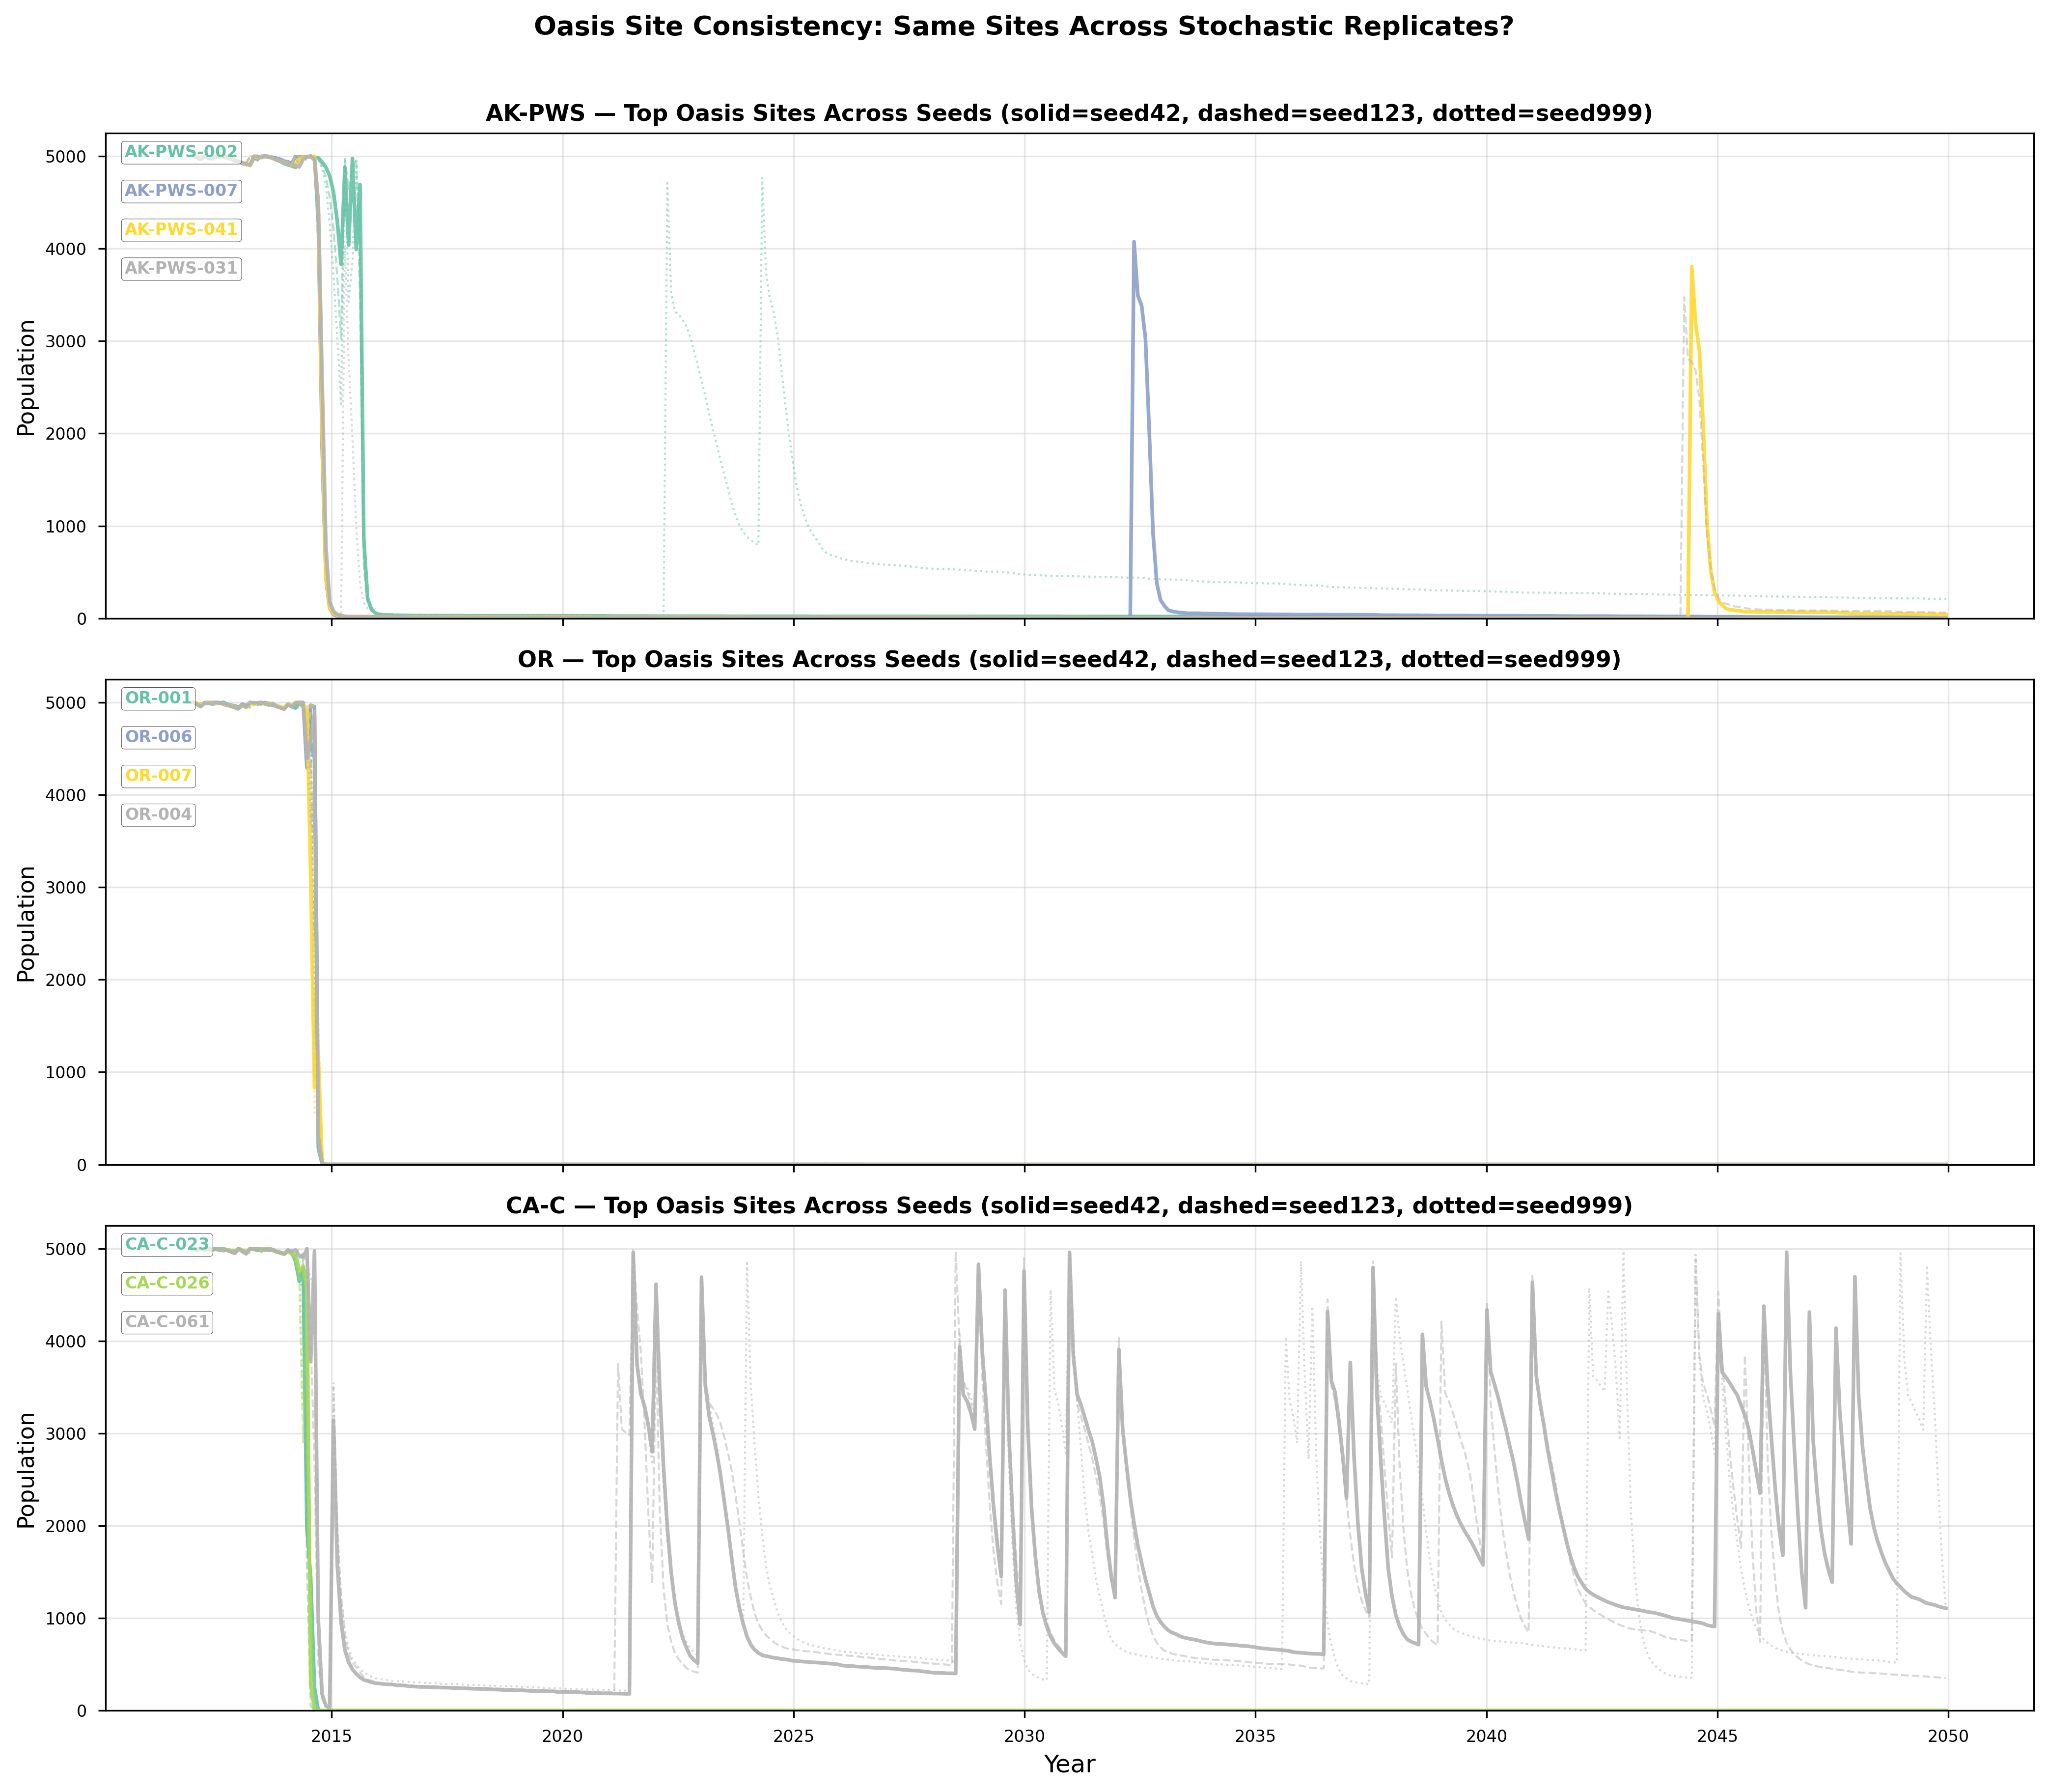
\includegraphics[width=0.90\textwidth]{figures/fig_oasis_consistency.png}
    \caption{Cross-seed consistency of oasis site identity in Oregon. Population trajectories of the top 5 Oregon sites under each of three independent random seeds. While the geographic \textit{zone} of oasis concentration is consistent (southern Oregon, 42--43\textdegree N), the specific sites that dominate vary across seeds: 13 different sites appear among the top 5 across three seeds, with only 2 appearing in more than one seed. Oasis geography is deterministic but oasis identity is stochastic, reflecting the role of sweepstakes reproductive success at small population sizes.}
    \label{fig:oasis_consistency}
\end{figure>

The conservation implication is important: \textbf{oasis sites cannot be
identified in advance from geographic or oceanographic data alone.}  While the
southern Oregon coast is consistently favorable, the specific sites that
sustain the population depend on stochastic reproductive events that are
inherently unpredictable.  Monitoring programs should therefore survey the
entire favorable zone rather than focusing on a few ``expected'' oasis sites.

% --- Figure: Oasis Consistency ---
\begin{figure}[!htbp]
    \centering
    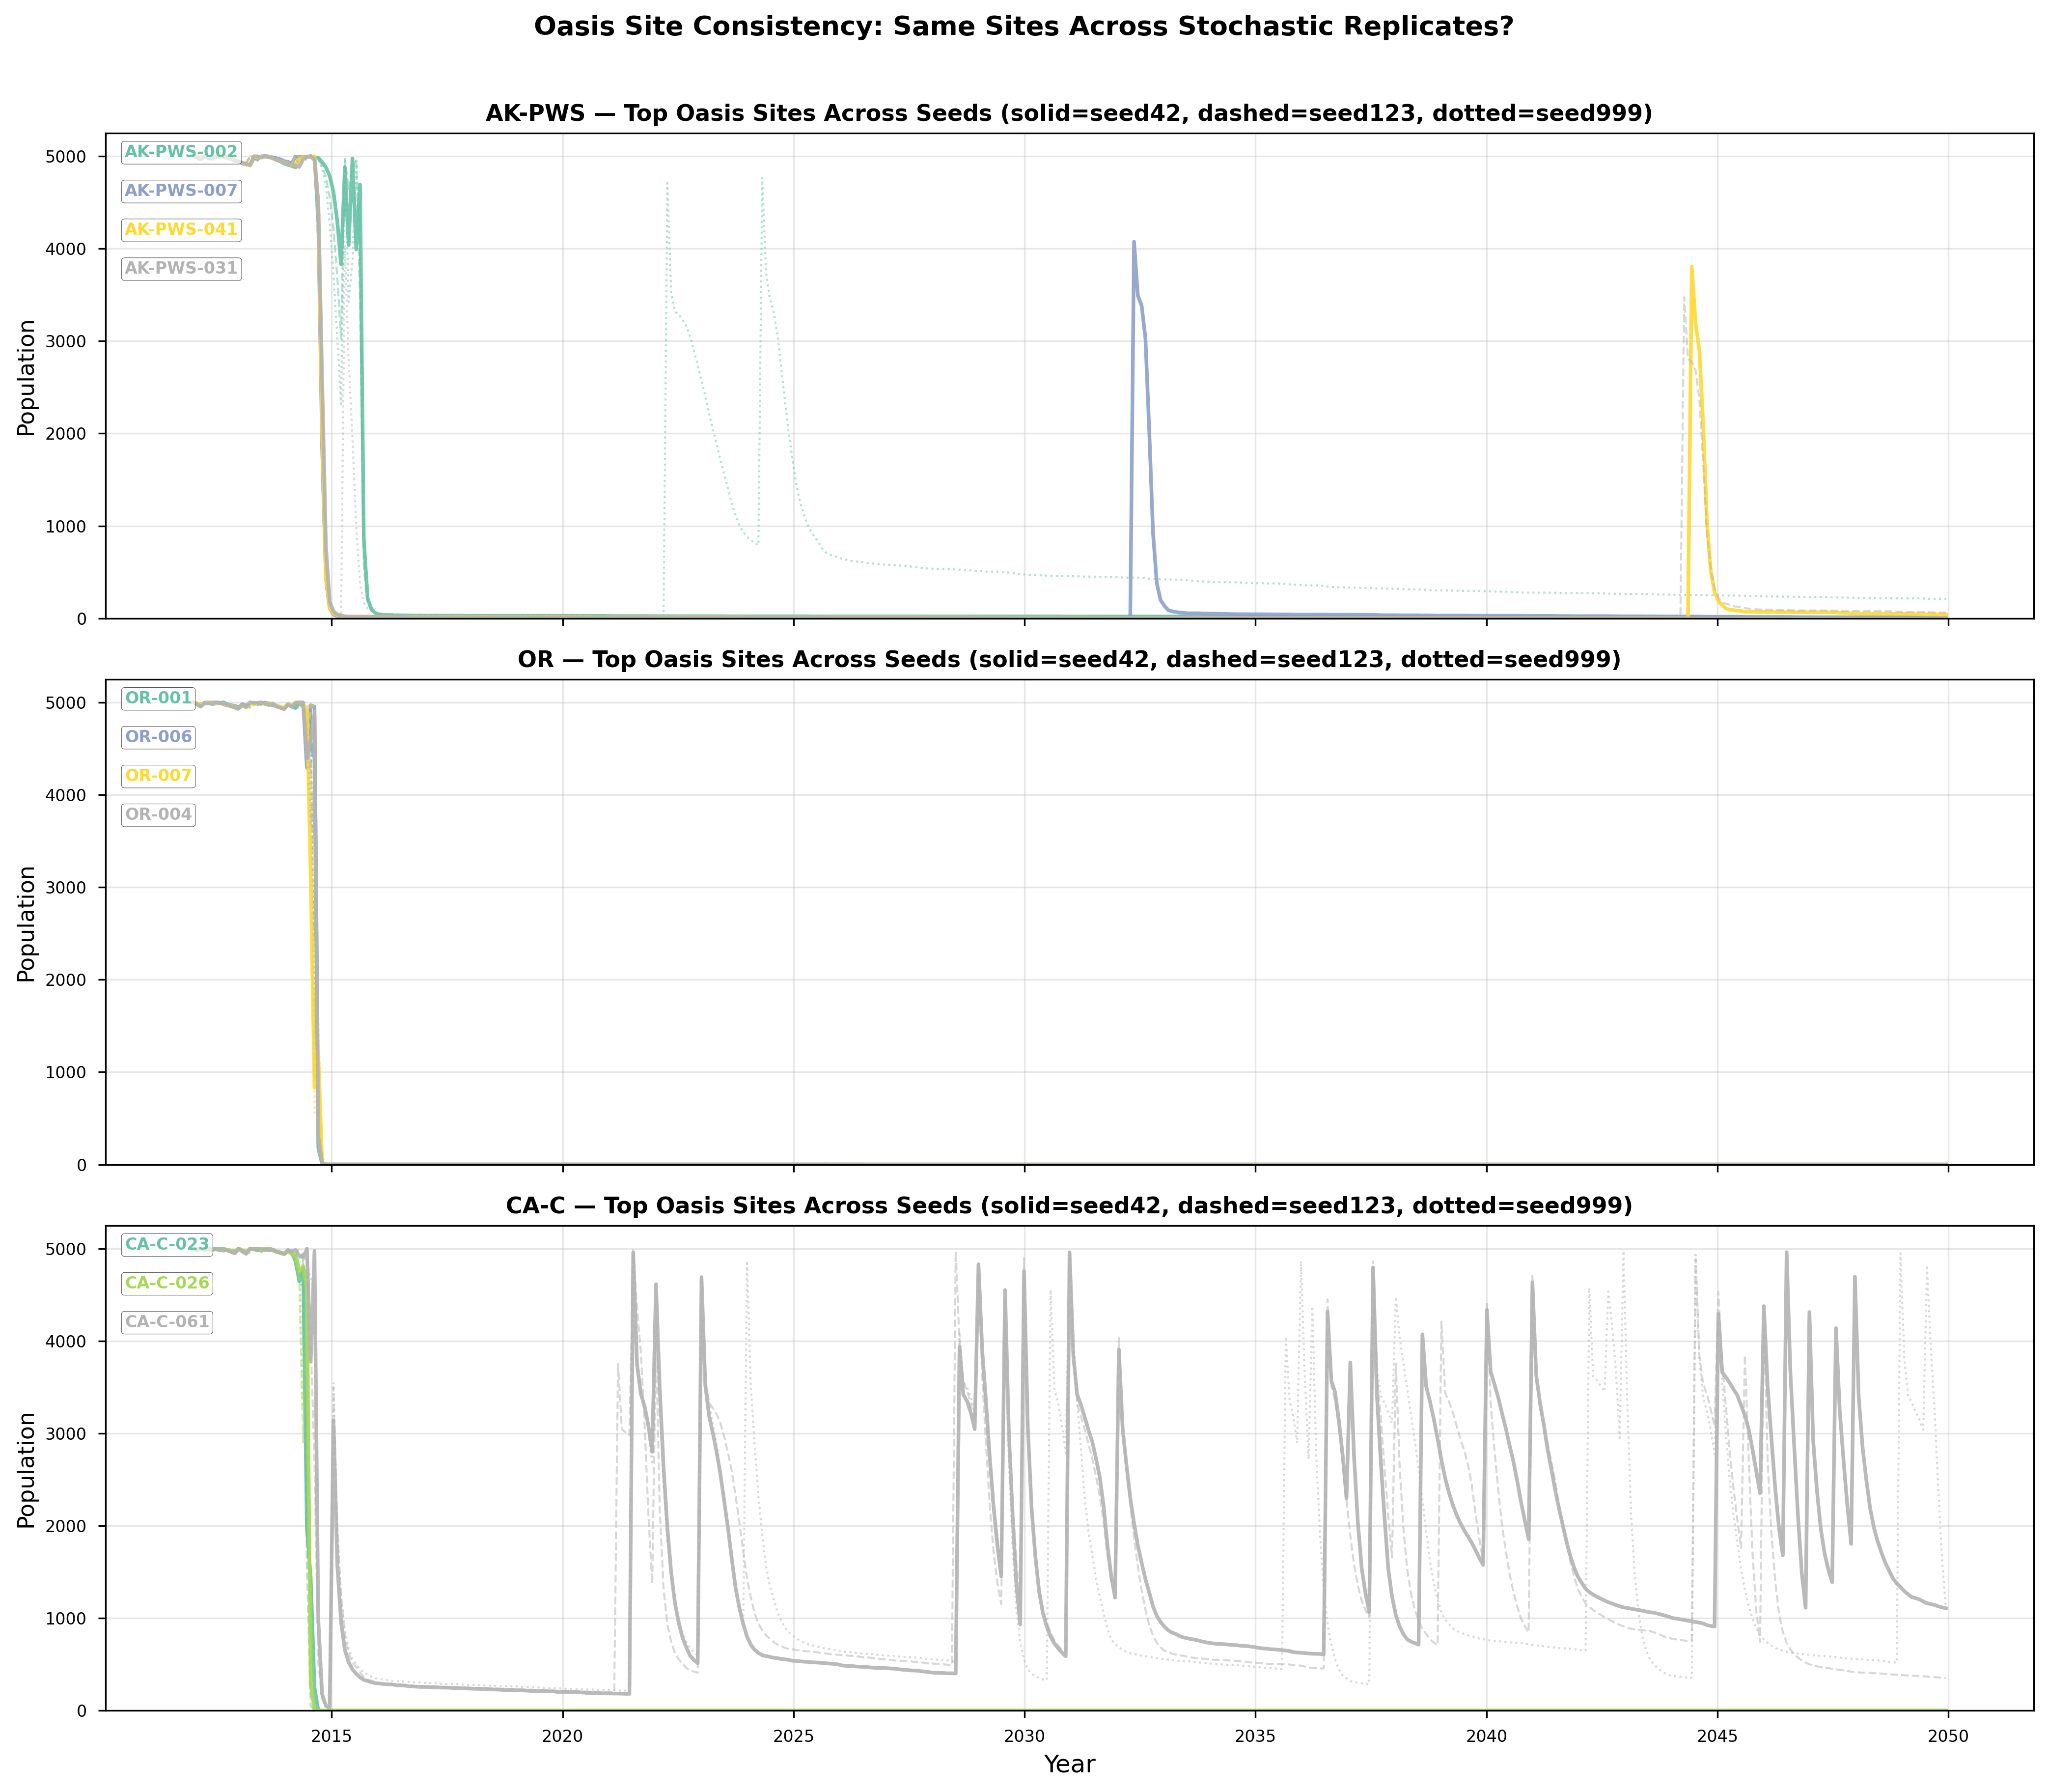
\includegraphics[width=0.90\textwidth]{figures/fig_oasis_consistency.png}
    \caption{Cross-seed consistency of oasis site identity in Oregon. Population trajectories of the top 5 Oregon sites under each of three independent random seeds. While the geographic \textit{zone} of oasis concentration is consistent (southern Oregon, 42--43\textdegree N), the specific sites that dominate vary across seeds: 13 different sites appear among the top 5 across three seeds, with only 2 appearing in more than one seed. Oasis geography is deterministic but oasis identity is stochastic, reflecting the role of sweepstakes reproductive success at small population sizes.}
    \label{fig:oasis_consistency}
\end{figure}

\subsubsection{Distributed Recovery in Alaska}

The Alaskan pattern is strikingly different.  In Prince William Sound (AK-PWS),
recovery is broad-based:

\begin{itemize}
  \item 37--38 of 43 sites retain population by 2050 (86--88\% of sites)
  \item The top 3 sites hold only 25--29\% of the regional population
  \item Gini coefficients remain moderate at 0.65--0.71
\end{itemize}

\noindent
Similarly, Fairweather North (AK-FN) maintains population across 37--40 of 40
sites (93--100\%), with Gini values of 0.63--0.66.  Alaska's distributed
persistence reflects two features of its thermal regime: (1) cold winter
temperatures suppress the pathogen broadly across all sites, not just at
favorable microhabitats; and (2) larval connectivity among nearby sites is
high, so recruitment events replenish depleted sites from the regional pool
rather than concentrating at a single source.

This contrast has practical implications for population monitoring.  In Alaska,
a random transect across the region will provide a representative estimate of
overall abundance.  In Oregon, a random transect will likely miss the oasis
sites entirely, producing an underestimate that could differ from the true
regional population by an order of magnitude.

\subsubsection{The Boom-Bust Cycle at Site Resolution}

The recruitment pulses described in Section~\ref{sec:trajectories} become
more dramatic when viewed at site resolution
(Figure~\ref{fig:site_decomposition}).  Oregon experiences repeated
boom-bust cycles (approximately every 3--4 years in the forecast period), and
each cycle is driven by a different combination of sites.  A typical boom
unfolds as follows:

\begin{enumerate}
  \item \textbf{Initiation (winter):} One or a few sites with surviving adults
    produce a successful larval cohort during the winter spawning season, when
    pathogen activity is suppressed by cold temperatures.
  \item \textbf{Amplification (spring):} Recruits grow rapidly and begin to
    reproduce themselves.  If multiple neighboring sites receive larvae from
    the same source (or from each other), the boom propagates along the coast.
  \item \textbf{Peak (late spring/early summer):} The regional population
    surges, sometimes by an order of magnitude within 6 months.  At peak,
    even a few thousand individuals across the region represent a dramatic
    improvement from the inter-boom nadir of a few hundred.
  \item \textbf{Crash (summer):} Rising SSTs reactivate the pathogen.
    The temporarily elevated host density amplifies the environmental pathogen
    pool through the shedding--infection positive feedback, and disease sweeps
    through the boom cohort.  Within 3--6 months, the regional population
    returns to near its pre-boom level.
\end{enumerate}

Importantly, the sites that initiate each boom are not always the same sites
that initiated the previous boom.  The stochastic nature of sweepstakes
reproduction, combined with the tiny population sizes between booms, means
that oasis identity shuffles between cycles.  However, the \textit{geographic
zone} from which booms originate remains consistent: the southern Oregon
coast, where the thermal regime most strongly favors winter recovery.

% --- Figure: Boom Decomposition ---
\begin{figure}[!htbp]
    \centering
    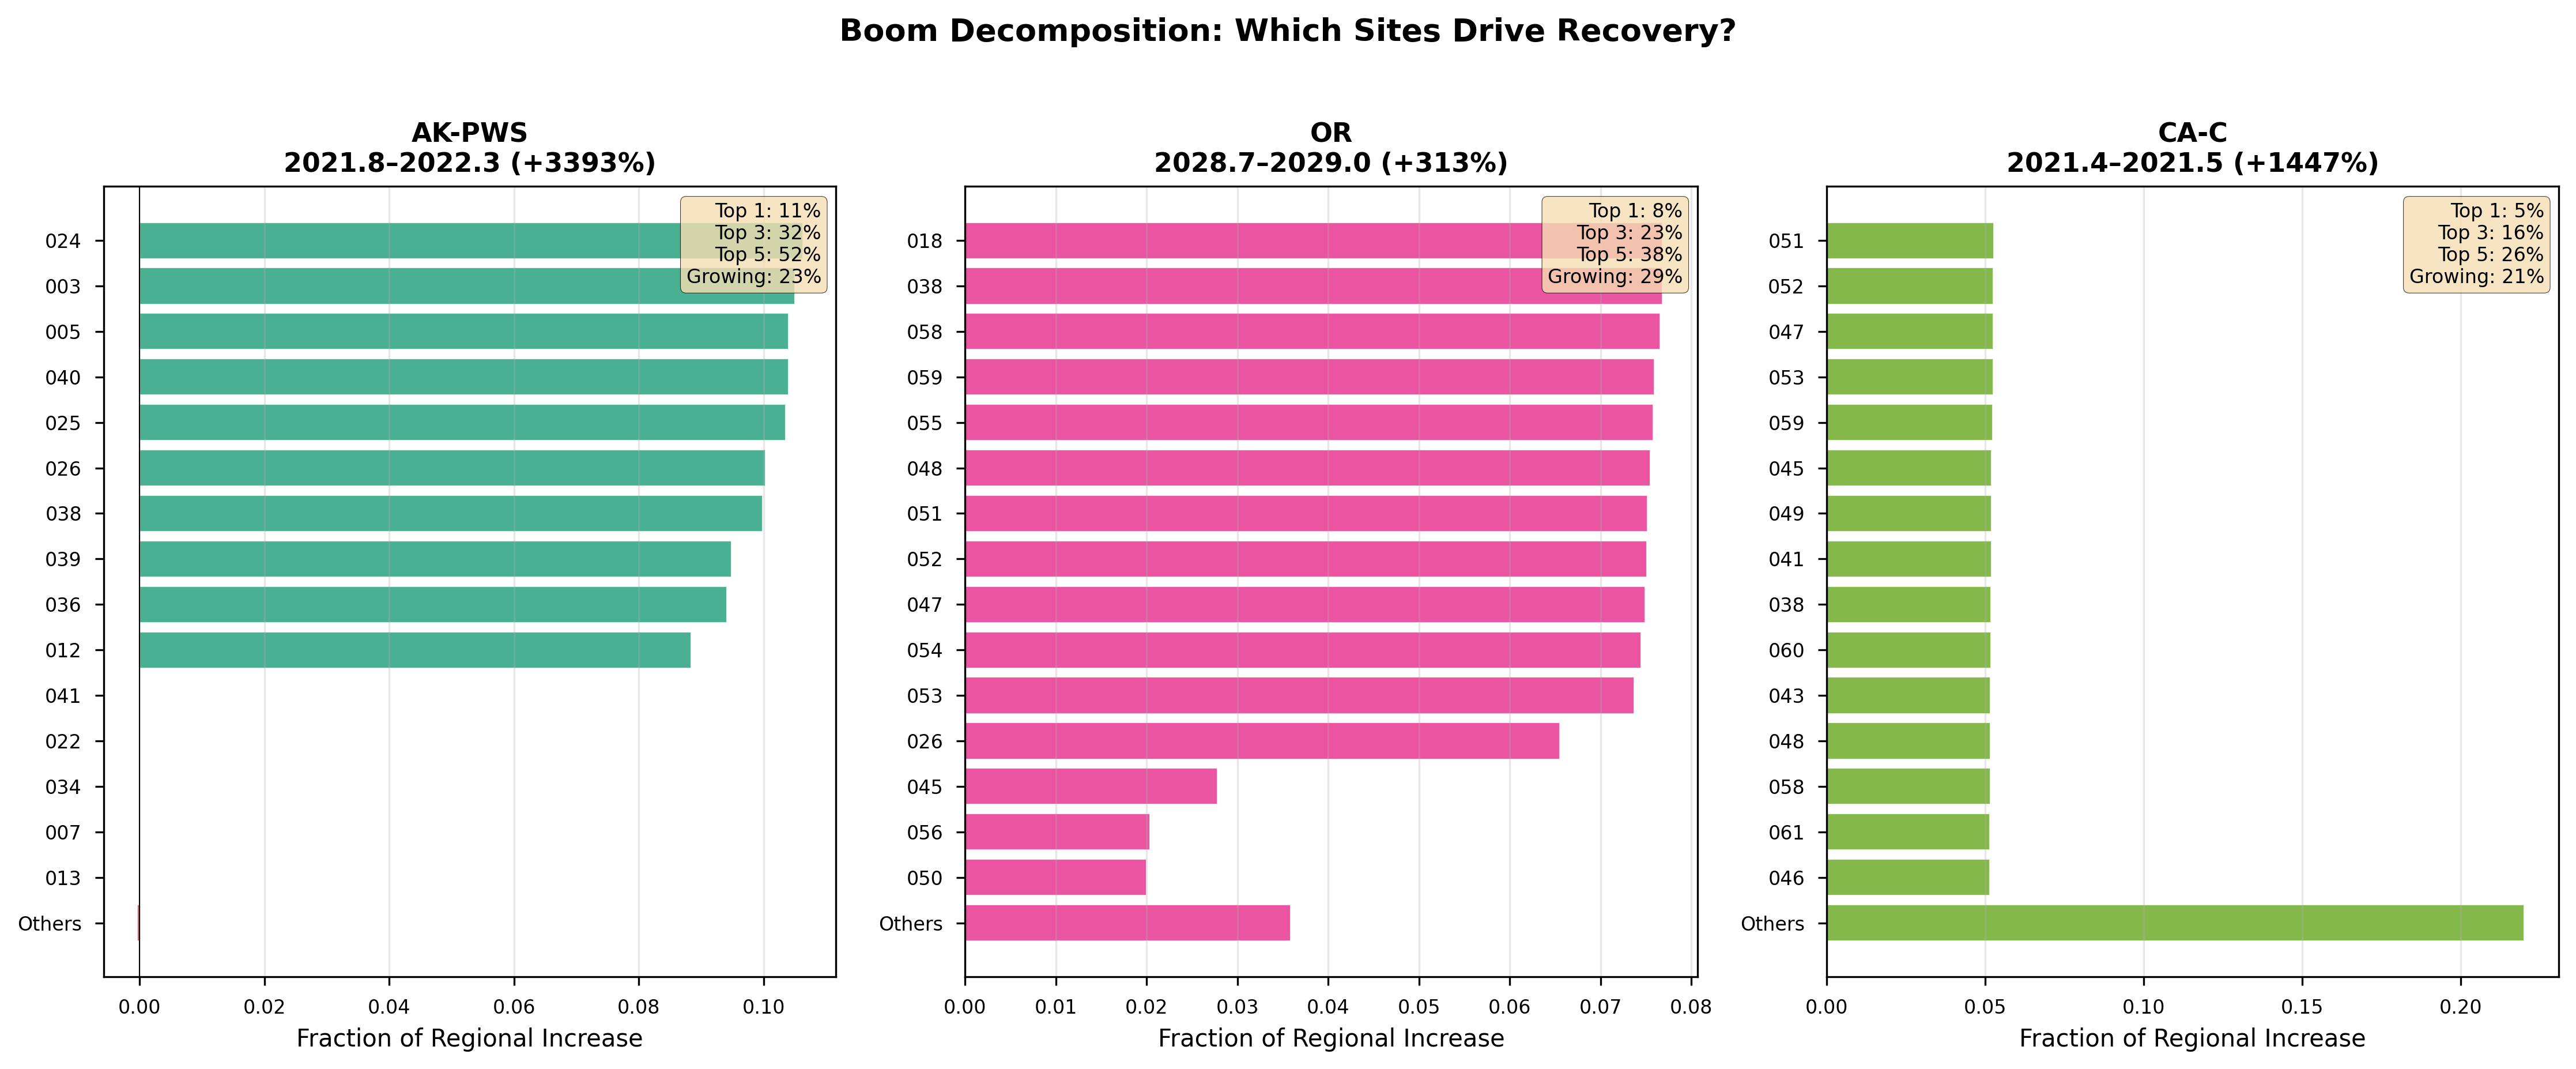
\includegraphics[width=0.85\textwidth]{figures/fig_boom_decomposition.png}
    \caption{Decomposition of selected recovery booms into individual site contributions. For each boom event (identified as periods where regional population increases by $>$50\% within 6 months), bars show each site's absolute contribution to the regional population increase, ranked from largest to smallest. In Oregon, a single site often contributes $>$40\% of the boom; in AK-PWS, the largest contributor accounts for only $\sim$10\%. This confirms the oasis-driven nature of Oregon recovery versus the distributed recovery in Alaska.}
    \label{fig:boom_decomposition}
\end{figure}

\subsubsection{Implications for Conservation}

The oasis analysis yields three actionable findings:

\begin{enumerate}
  \item \textbf{Oregon's ``recovery'' is fragile.}  A regional recovery
    rate of 17.6\% sounds encouraging, but when this population is
    concentrated in 2--3 sites with $\sim$80\% of the total, it is
    vulnerable to a single localized catastrophe (an oil spill, a hypoxia
    event, a point-source pollutant) that could eliminate the majority
    of the regional population in a single event.

  \item \textbf{Reintroduction should target oasis zones, not specific
    sites.}  Because oasis identity is stochastic but oasis geography is
    consistent, captive breeding releases should distribute individuals
    across the favorable zone (e.g., multiple sites along the southern
    Oregon coast) rather than concentrating them at a single site that
    may or may not become a successful oasis.

  \item \textbf{Northern populations are more resilient to local
    disturbance.}  The distributed persistence pattern in Alaska means
    that losing any single site has a small impact on regional population
    viability.  This inherent redundancy makes Alaskan populations better
    candidates for long-term self-sustaining recovery, even though their
    absolute numbers are currently lower than Oregon's.
\end{enumerate}
